\documentclass[a4paper,twoside]{article}
\usepackage{graphicx}
\usepackage{url}
\usepackage{listings}
\usepackage{float}
\usepackage[width=0.89\textwidth]{caption}

\usepackage[natbib=true,
    style=numeric,
    sorting=none,
    backend=biber]{biblatex}
\addbibresource{o2bibliography.bib}

\usepackage{lineno}
\linenumbers

\def\O2{O$^2$}

\begin{document}

\title{ALICE \O2 data model proposal}

\author{Mikolaj Krzewicki \and Sylvain Chapeland \and Roberto Divia \and Matthias Richter \and David Rohr}
\date{
for the CWG4 data model group.\\[2ex]
\today
}

\maketitle

\abstract{This note presents a proposal for the ALICE \O2 data model. A base data layout and metadata format that allow for
efficient resource use are proposed. Application of the data model to online/offline data processing and quality control is discussed.}

\section{Introduction}

The ALICE online-offline (\O2) computing system \cite{o2tdr,o2} is a computing facility and a software framework designed for the processing of the ALICE data in the upcoming LHC Run 3.
The design aims at high data throughput and parallelism using a multiprocess model.
It does not, however, exclude the use of multithreading and other forms of concurrent processing inside of individual processes.

The data exchange between processes running within the \O2 system (called \O2 devices) is taken care of by the ALICE-FAIR (Alfa ) framework \cite{alfa}. Since this is the only communication mechanism foreseen for data exchange, it effectively serves the role of an API between the devices.
The Alfa framework provides data transport and synchronisation primitives via the FairMQ message queue library. FairMQ messages consist of raw memory buffers which are asynchronously queued and atomically delivered.

The online data processed by the \O2 system consists of a set of data buffers originating from the detector hardware (raw data) and the processing devices (derived data). The data fragments are logically grouped into (sub-) time frames. A (sub-) time frame contains raw data associated to a period of data taking (typically several tens of ms, as dictated by the heartbeat trigger \cite{O2readout}) and/or the results of the processing of these data. In addition any data that might be necessary to describe and qualify the data set can be added to the logical group.

In the unified online-offline software model also derived data is handled within the same software framework. \O2 devices dedicated to quality control (QC) and physics analysis tasks should use the same set of interfaces as pure online components. The requirements for the data used in these tasks tend to be different from the online components: high level abstractions and ease of use (of e.g. ROOT\cite{root} objects) is sometimes preferred to high performance low-level data structures. Transparent support for high level data structures is part of the proposed data model.

A single time frame data volume is expected to be of the order of tens of gigabytes. The data model facilitates communication approaches that minimize resource use, i.e. avoid unnecessary copies of data.

In order to assure consistent navigation within a time frame, each data fragment is described by a small metadata block containing the information about the content type of the payload, it's origin and serialization strategy.
In addition, the metadata block can be extended by the processing devices with additional information without the need to modify the payload.

\section{Message queue based communication}

Vectored IO (also referred to as scatter/gather IO) is an important feature when dealing with multiple data buffers as it allows, in principle, to avoid the cost associated with serializing data into a single IO buffer.
Vectored IO is provided in FairMQ in the form of multi-part messages. A multi-part message consists of multiple independent buffers and is delivered atomically as a whole while preserving the ordering of the buffers.

The multi-part approach, in addition to minimizing the resource strain associated with IO buffer construction, also by construction reduces the need for (re-)synchronisation and event building; data fragments once associated to a single time frame remain that way throughout the entire chain regardless of the networking topology. Another benefit is that additional data parts can be attached or removed by other processing devices without copy overhead at any point of the processing chain.

\section{\O2 Message structure}

The \O2 message consists of a sequence of metadata-payload pairs contained within a multi-part message. Each payload is described by metadata contained in a separate message part. Since FairMQ preserves the ordering of the parts, the natural choice is to precede each data part with the associated metadata part in the message, as illustrated in figure \ref{fig:o2message}. 

\begin{figure}[h]
  \centering
  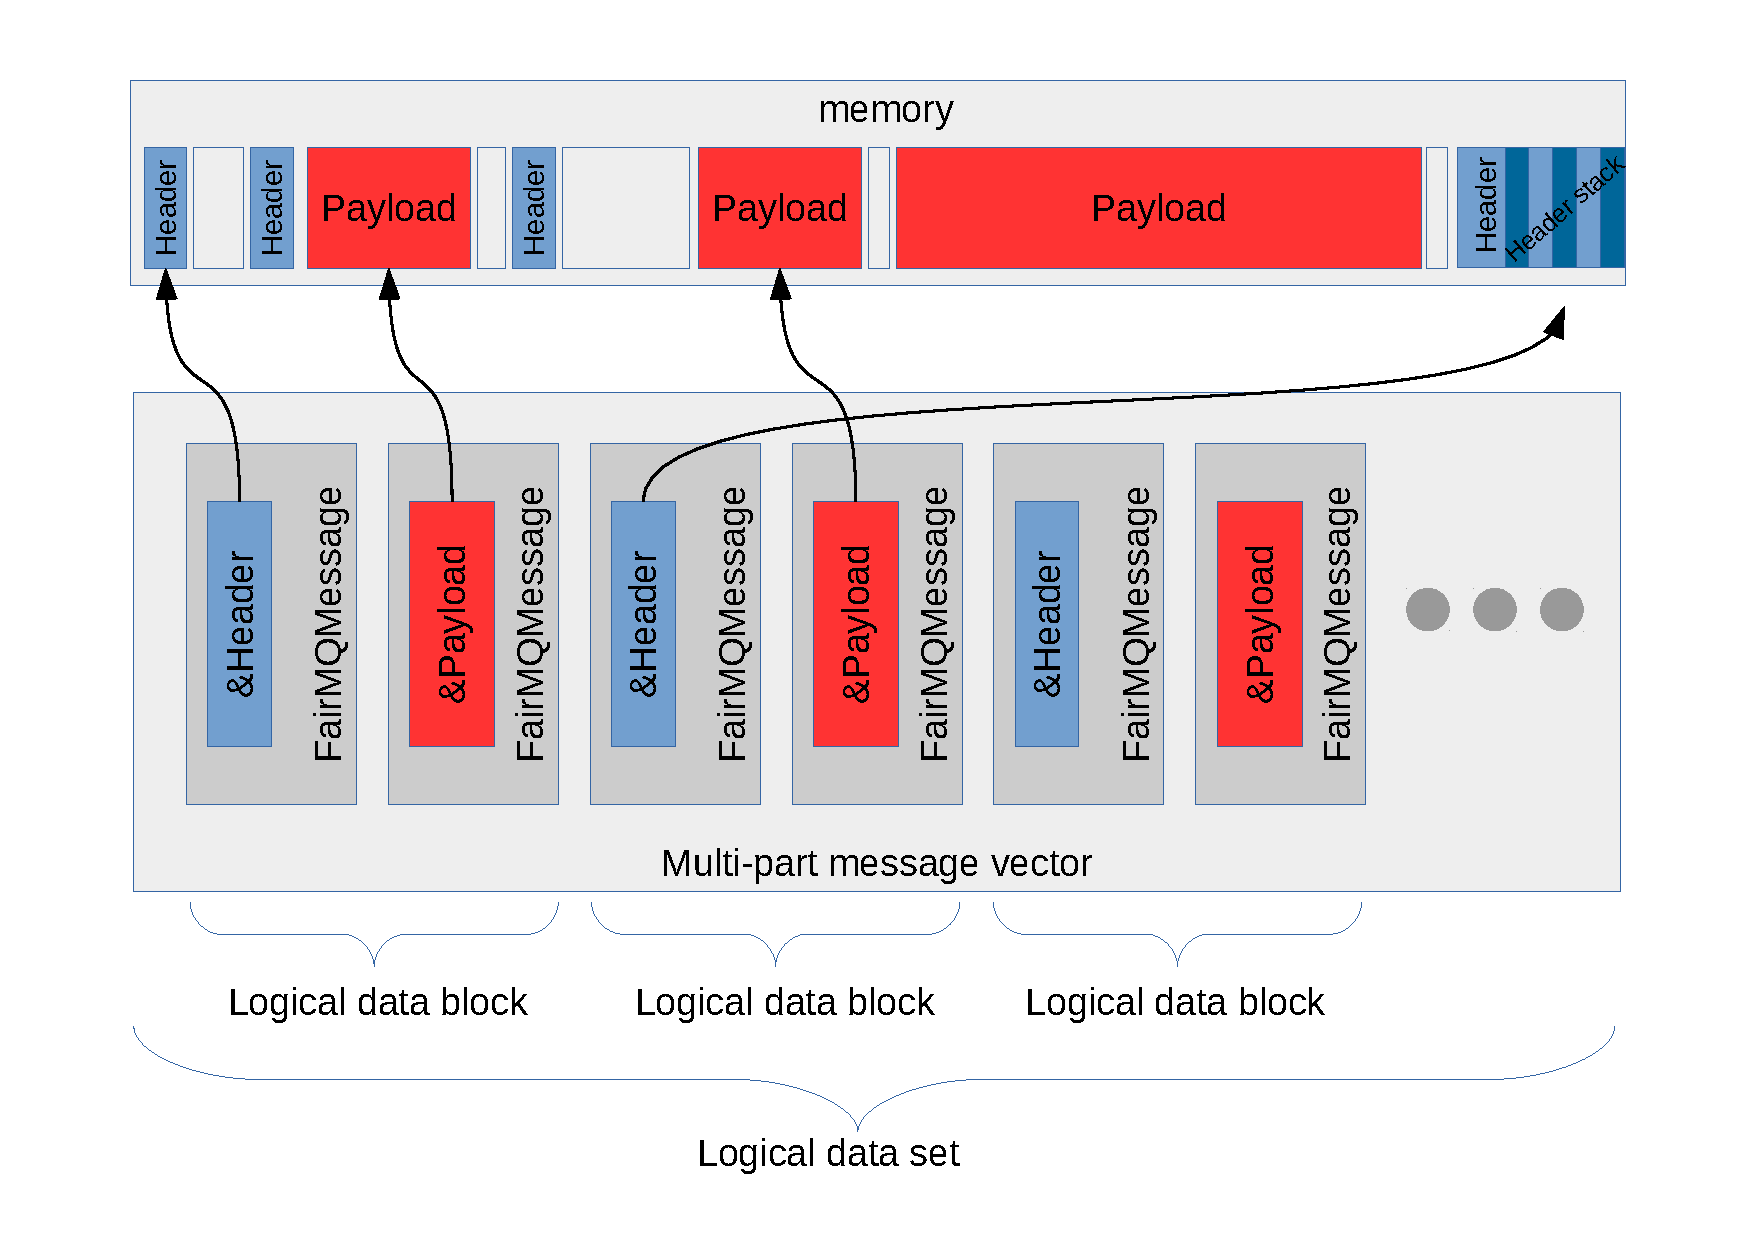
\includegraphics[width=0.89\textwidth]{multipartO2message.pdf}
  \caption{The \O2 message structure. Logical data blocks consisting of payload and metadata parts are contained in a multi-part FairMQ message (bottom). The buffers associated to the message parts do not have to be contiguous in memory (top).}
  \label{fig:o2message} 
\end{figure}

Storing the metadata and data payload in separate buffers offers several advantages:

\begin{itemize}
  \item Since the metadata is separated from the payload already at transport level, efficient navigation is possible as only the (small) metadata parts need to be inspected.
  \item The size of the metadata buffer is not fixed enabling a scheme with flexible metadata content.
  \item The content of the data buffers, once produced by the hardware or a processing device, is immutable to other devices. Since the metadata is encapsulated in a separate buffer, it becomes possible to add additional information to the metadata with minimal cost and without modifying the payload downstream from the data producer.
\end{itemize}

\section{Metadata format}

The O2 metadata consists of a contiguous buffer containing a sequence of headers (header stack).
The byte representation of a header consists of a user defined body following a BaseHeader struct containing fields needed to:
\begin{itemize}
  \item Verify that the following data (header body) belongs to an \O2 header.
  \item Define the size of the entire header.
  \item Flag whether another header follows this one in the stack.
  \item Verify the version of the header.
  \item Signal the type of the header.
  \item Signal the packing/serialization scheme of the metadata body carried by the header.
\end{itemize}

The header stack should contain at least the standard DataHeader struct describing the basic payload properties common to all payloads. The DataHeader representation starts with the BaseHeader followed by bytes representing:
\begin{itemize}
  \item The functional data description uniquely determining the data type contained in the payload.
  \item The payload serialization method (e.g. ROOT, FlatBuffers, none) complementing the data description field.
  \item The origin of the data to identify the producer (e.g. detector system or a software subsystem).
  \item A data type dependent 64 bit specification. This can be used by the detectors to store e.g. the fine grained equipment ID like the link number for raw data or cluster finder instance for clusters\footnote{Based on HLT experience: most data types use some kind of fine grained ID. This field has been added here to avoid the overhead of a full header for what in most cases would be just one (64 bit) field.}.
  \item The payload buffer size\footnote{This is not strictly necessary online as the transport framework keeps track of the buffer sizes. Keeping this information is the header is useful for persistent storage and debugging purposes.}.
\end{itemize}

Other headers can be defined similarly to DataHeader and included in the header stack. Examples include trigger information for triggered detector data, object name for ROOT objects used in quality control etc.

\subsection{Header memory layout}
The memory layout of the DataHeader struct is illustrated by the following definition:

\lstset{language=C++
%,
%                keywordstyle=\color{blue},
%                stringstyle=\color{red},
%                commentstyle=\color{green},
%                morecomment=[l][\color{magenta}]{\#}
}
\begin{lstlisting}
struct BaseHeader
{
  uint32_t  magicString;
  uint32_t  headerSize;
  uint32_t  flags;
  uint32_t  headerVersion;
  uint64_t  headerDescription;
  uint64_t  headerSerialization;
};

struct DataHeader : public BaseHeader
{
  uint64_t dataDescription[2];
  uint32_t dataOrigin;
  uint32_t reserved;
  uint64_t payloadSerializationMethod;
  uint64_t subSpecification;
  uint64_t payloadSize;
};

\end{lstlisting}

\subsection{Header interface}

Data members representing (in principle) arbitrary integers (headerSize, payloadSize, subSpecification) or bitfields (flags) are directly accessible and settable as integers.

Access to other members is protected by strongly typed interfaces. Initialization can only be performed using predefined constants, consistency is then assured by the type system at compile time.

Access to header information contained in a metadata buffer is also implemented in a type safe way.

\subsubsection{Example}
The user may check if a given buffer contains the desired header information in a type safe way. If the desired header is of type DataHeader, a call to:
\begin{lstlisting}
DataHeader* header = Header::get<DataHeader>(buffer);
\end{lstlisting}

will yield a valid pointer if a header of type DataHeader is part of the header stack inside the buffer pointed to by the buffer pointer.

\section{Data formats}

The \O2 data model does not impose any limitations on the data types exchanged between devices. The only constraint from the data transport layer is that the trasported payload must be contiguous in memory. For higher level data types it usually means that they need to be serialized which penalizes performance (to a varying degree). A trade off has to be made between flexibility and performance based on the use case for a particular data type.

\subsection{Data in memory}
The recommendation is to use flat POD data types where performance and/or memory usage is critical. Flat data means natually contiguous data that does not require a serialization step and does not contain any process specific run time dependent information like virtual function table pointers or pointer/reference members.

Outside of the critical path where relatively a low volume of data needs to be transported between devices, serialization schemes possibly impose acceptable overhead. The data model supports serialization schemes and facilitates the handling of serialization and deserialization of data transparently to user code.

\subsection{Raw data formats}
Raw data formats will be determined by the readout hardware of the detectors.

\subsection{Reconstructed data formats}
Reconstructed data 

\subsection{Persistent storage of time frame data}
The in-memory data representation of header and payload buffers contains enough information to be stored on-disk directly as a sequence of buffers. The data represented by POD data are, however, not suitable for long term storage and need to be transformed to a portable and extensible format.

In the modular \O2 design only a dedicated device would handle persistent storage making the translation steps from and to peristent storage format transparent to other devices which only need to deal with the in-memory format.

\subsection{Quality control formats}
The Quality control (QC) devices will produce ROOT based data.

\subsection{AOD format}
The contents of the AOD data used for end user physics data analysis is being prepared by the physics community. Work is being done on developing the in-memory layout that will support efficient processing, pruning and distribution in the message based \O2 environment. The struct-of-arrays approach that is currently investigated also allows for transparent extensions of the data content. The persistent storage of AOD still needs to be investigated.

\section{Interfaces}
The base functionality of a device running in the \O2 system is contained in the FairMQDevice class. This is a generic class providing all the necessary logic to support the \O2 system and data model, like control abstractions, a state machine and multi-part messaging. FairMQ support for the multi-part messaging is, however, unaware of the \O2 specific message layout. In order to enforce a consistent handling of the metadata the necessary interface is implemented on top of FairMQDevice as O2device.

Each device in the \O2 system should inherit from the O2device class in order to be able to use the data model. Interfaces are provided that insure consistency in the handling of the data and associated metadata.

\subsection{Examples}
To construct a message, the AddMessage(...) family of methods should be used to insure correct association of metadata to payloads, e.g. in the simplest case:
\begin{lstlisting}
bool AddMessage( FairMQParts& message,
                 AliceO2::Header::Block&& headerStack,
                 FairMQMessagePtr payloadPart );
\end{lstlisting}
where in a single call the header stack to payload association is made and data is appended to the message.

After the message is constructed a call to the standard FairMQ send method suffices:
\begin{lstlisting}
int64_t Send( const FairMQParts& parts,
              const std::string& channel );
\end{lstlisting}
This queues the entire message for atomic delivery via a specified data channel.

For decoding the message on the receiving end functionality is provided to access the metadata and it's associated payload in a consistent way. The user implements a function that takes the metadata and the payload buffers as input, and uses that function via e.g. a call to:
\begin{lstlisting}
template <typename T>
bool ForEach(
       O2message& parts,
       bool (T::*memberFunction)(
         const byte* headerBuffer, size_t headerBufferSize,
         const byte* dataBuffer, size_t dataBufferSize
       )
     );
\end{lstlisting}
Inside the user provided function the metadata and the payload are decoded and processed.

\printbibliography

\end{document}
